\documentclass[runningheads]{llncs}

\usepackage[T1]{fontenc}
\usepackage{graphicx}
\usepackage{amsmath,amssymb,amsfonts}
\usepackage{booktabs}
\usepackage{multirow}
\usepackage{xcolor}
\usepackage{algorithm}
\usepackage{algorithmic}
\usepackage{hyperref}

\begin{document}

\title{Ollivier--Ricci Curvature as a Landscape Metric\\for Discrete Combinatorial Optimization}
\titlerunning{ORC as a Landscape Metric for Discrete Optimization}

\author{Hordoan Roberto Sergiu}
\authorrunning{Hordoan Roberto Sergiu}
\institute{University Babes-Bolyai, Cluj-Napoca, Romania}

\maketitle

\begin{abstract}
Understanding the structure of fitness landscapes is central to explaining and predicting the performance of metaheuristic optimizers.
Existing landscape metrics---such as fitness-distance correlation~(FDC) and autocorrelation length---capture global statistical properties but are blind to \emph{local geometric structure} at local optima.
We introduce \emph{Ollivier--Ricci curvature}~(ORC), a discrete analogue of Ricci curvature from Riemannian geometry, as a new landscape metric for combinatorial optimization.
ORC measures how the neighborhoods of two adjacent solutions diverge or converge, providing a principled way to detect \emph{inter-basin saddle directions} at local optima.
We prove that on the $N$-dimensional binary hypercube ($N \ge 4$) with a neighborhood-aware transport cost, every local optimum whose smallest fitness gap satisfies an explicit bound possesses at least one negative-ORC edge---a condition met at 100\% of tested local optima.
Through experiments on NK~landscapes ($N \in \{16,20\}$, 260~instances), W-model benchmarks (6~epistasis levels, 180~instances), and NAS-Bench-201 (15{,}625~architectures), we show that:
(1)~following the most negative ORC direction leads to a better local optimum \textbf{2.0$\times$ more often} than following a random direction (e.g., 59.6\% vs.\ 31.6\% on NK $K\!=\!4$);
(2)~ORC-based features correlate more strongly with hill-climbing difficulty ($\rho = {-}0.670$) than FDC ($\rho = 0.276$) or autocorrelation length ($\rho = 0.543$); and
(3)~these results hold at both $N\!=\!16$ and $N\!=\!20$ scales.
Our results establish ORC as a complementary landscape metric that reveals basin connectivity structure invisible to existing approaches, including local optima networks.
\end{abstract}

\keywords{Fitness landscape analysis \and Ollivier--Ricci curvature \and Discrete optimization \and NK~landscapes \and Basin structure}


% ===================================================================
\section{Introduction}
\label{sec:intro}
% ===================================================================

Fitness landscape analysis (FLA) is fundamental to understanding why certain optimization problems are hard for specific algorithms and how to select appropriate solvers~\cite{pitzer2012comprehensive}.
A rich toolkit of landscape metrics has been developed, including fitness-distance correlation (FDC)~\cite{jones1995fitness}, autocorrelation functions~\cite{stadler1996landscapes}, information content~\cite{vassilev2000information}, and exploratory landscape analysis (ELA) features~\cite{mersmann2011exploratory}.
These metrics characterize \emph{global} properties of the landscape---its ruggedness, smoothness, and correlation structure---and have proven valuable for algorithm selection and configuration~\cite{kerschke2019automated}.

However, existing metrics share a fundamental limitation: they capture statistical summaries of the landscape but are blind to \emph{local geometric structure} at and around local optima.
Consider two landscapes with identical FDC and autocorrelation profiles but different basin connectivity: in one, local optima are isolated; in the other, specific directions at local optima lead through ``saddle regions'' to better basins.
No existing metric distinguishes these cases, yet the distinction is precisely what determines whether local-search-based algorithms can escape suboptimal basins.

Local optima networks (LONs)~\cite{ochoa2008first,ochoa2017understanding} represent basin connectivity as a graph whose nodes are local optima and whose edges encode perturbation-based transitions.
While LONs capture the \emph{existence} of inter-basin transitions, they do not provide \emph{directional} information: at a given local optimum, which specific neighbor should be followed to escape the current basin?
Furthermore, LON edges are defined by stochastic perturbation followed by hill climbing, making the construction expensive and sensitive to the choice of perturbation strength.

We address these gaps by introducing \emph{Ollivier--Ricci curvature}~(ORC)~\cite{ollivier2009ricci} as a new landscape metric for discrete optimization.
ORC is a discrete analogue of Ricci curvature from Riemannian geometry that measures how the neighborhood distributions of two adjacent nodes diverge or converge.
Negative ORC along an edge indicates that the neighborhoods are ``spreading apart''---precisely the geometric signature of a saddle region between basins of attraction.
Crucially, ORC is computed \emph{locally} at a single node and provides a \emph{signed scalar per direction}, enabling principled ranking of escape directions.

\textbf{Contributions.} We make four contributions:
\begin{enumerate}
\item We formalize ORC on discrete search graphs with a neighborhood-aware transport cost (Section~\ref{sec:method}).
\item We prove an explicit sufficient condition for negative ORC at local optima on Hamming graphs: $\Delta < (N\!-\!3)/((N\!+\!1)\gamma)$ (Theorem~\ref{thm:negative}, Section~\ref{sec:theory}), verified at 100\% of tested optima.
\item We demonstrate through extensive experiments on three benchmark families (530+ instances) that the most-negative-ORC direction leads to a better local optimum \textbf{significantly more often} than a random direction---up to 2.7$\times$ more frequently (Section~\ref{sec:results}).
\item We show that ORC-based features correlate more strongly with algorithm difficulty than classical metrics including FDC, autocorrelation length, and information content (Section~\ref{sec:results}).
\end{enumerate}


% ===================================================================
\section{Background and Related Work}
\label{sec:background}
% ===================================================================

\subsection{Fitness Landscapes and Search Graphs}

A \emph{fitness landscape} is a triple $(S, \mathcal{N}, f)$ where $S$ is a set of candidate solutions, $\mathcal{N}: S \to 2^S$ defines a neighborhood structure, and $f: S \to \mathbb{R}$ is a fitness function~\cite{stadler1996landscapes}.
For discrete optimization, $S$ is typically a set of binary or $k$-ary strings, and $\mathcal{N}$ defines adjacency via single-position mutations (e.g., bit-flip or operation swap).
A solution $x^* \in S$ is a \emph{local optimum} (for minimization) if $f(x^*) \le f(y)$ for all $y \in \mathcal{N}(x^*)$.
The \emph{basin of attraction} of $x^*$ is the set of all solutions from which greedy hill climbing converges to~$x^*$.

\subsection{Classical Landscape Metrics}

\textbf{Fitness-distance correlation (FDC)}~\cite{jones1995fitness} measures the Pearson correlation between $f(x)$ and $d(x, x^*_{\mathrm{global}})$ for sampled solutions $x$, where $d$ is the graph distance.
High positive FDC (for minimization) indicates that fitness improves toward the global optimum, suggesting the landscape is ``easy'' for local search.

\textbf{Autocorrelation length}~\cite{stadler1996landscapes} is the lag at which the autocorrelation of fitness values along random walks drops below $1/e$.
Short correlation length indicates a rugged landscape where fitness values change rapidly between neighbors.

\textbf{Information content}~\cite{vassilev2000information} captures the entropy of fitness-change patterns (improving, neutral, worsening) along random walks.
High entropy indicates an unpredictable, rugged landscape.

\textbf{Basin entropy} measures the Shannon entropy of the basin-size distribution.
Low entropy (one dominant basin) suggests easy landscapes; high entropy (many small basins) suggests difficult ones.
Unlike the other metrics, basin entropy requires exhaustive landscape enumeration.

These metrics are informative but capture \emph{global statistical averages}.
They do not characterize the geometry at specific local optima or identify \emph{which direction} to follow to escape a basin.

\subsection{Local Optima Networks}
\label{sec:lon}

Local optima networks (LONs)~\cite{ochoa2008first,ochoa2014local,ochoa2017understanding} provide a compressed representation of landscape structure.
A LON is a directed graph where nodes are local optima and edges represent transitions discovered by perturbation operators followed by hill climbing.
Specifically, an edge from optimum $x^*_i$ to $x^*_j$ exists if perturbing $x^*_i$ (e.g., flipping $d$ random bits) and then hill-climbing reaches~$x^*_j$.
LON features such as the number of nodes, number of funnels, and autocorrelation of the LON itself have proven predictive of search difficulty~\cite{ochoa2017understanding}.

While LONs and ORC both capture inter-basin connectivity, they differ in three ways:
(1)~LON edges are discovered by stochastic perturbation + hill climbing; ORC is computed deterministically in $O(k^4)$.
(2)~LON edges are binary; ORC provides a signed scalar per neighbor, enabling ranking.
(3)~ORC requires only 2-hop information; LON construction depends on perturbation distance.
ORC thus provides a fine-grained, deterministic view complementing the coarser, stochastic LON view.

\subsection{Ollivier--Ricci Curvature on Graphs}

Ollivier~\cite{ollivier2009ricci} introduced a notion of Ricci curvature for metric spaces equipped with Markov chains.
For a graph $G = (V, E)$ with metric $d$, the ORC of edge $(x, y) \in E$ is:
\begin{equation}
\label{eq:orc}
\kappa(x, y) = 1 - \frac{W_1(\mu_x, \mu_y)}{d(x, y)}
\end{equation}
where $\mu_x, \mu_y$ are probability distributions supported on the neighborhoods of $x$ and $y$ (including themselves), and $W_1$ denotes the Wasserstein-1 (earth mover's) distance~\cite{villani2009optimal} with respect to $d$.

Intuitively:
\begin{itemize}
\item $\kappa > 0$ (positive curvature): neighborhoods overlap and the space ``contracts'' along $(x,y)$---analogous to a sphere.
\item $\kappa = 0$ (flat): neighborhoods are optimally aligned---analogous to flat space.
\item $\kappa < 0$ (negative curvature): neighborhoods diverge and the space ``spreads'' along $(x,y)$---analogous to a saddle.
\end{itemize}

ORC has been applied to community detection in networks~\cite{ni2019community}, where negative curvature identifies ``bridges'' between communities; to cancer network analysis~\cite{sandhu2015graph}; and to understanding over-squashing in graph neural networks~\cite{topping2022understanding}.
To our knowledge, ORC has not previously been used for fitness landscape analysis.


% ===================================================================
\section{ORC as a Landscape Metric}
\label{sec:method}
% ===================================================================

\subsection{Fitness-Lifted ORC on Search Graphs}

For each node $x$, the support distribution $\mu_x$ is the uniform distribution over $\{x\} \cup \mathcal{N}(x)$.
On a $k$-regular graph, $|\mathrm{supp}(\mu_x)| = k + 1$ for all $x$.

To compute $W_1(\mu_x, \mu_y)$ for an edge $(x,y)$, we define a \emph{neighborhood-aware transport cost} reflecting the overlap structure of the supports $A = \mathrm{supp}(\mu_x)$ and $B = \mathrm{supp}(\mu_y)$.
Formally, for $a \in A$ and $b \in B$:
\begin{equation}
\label{eq:lifted}
c(a, b) = \delta(a, b) + \gamma \cdot |f(a) - f(b)|
\end{equation}
where $\gamma \ge 0$ controls the fitness sensitivity and the \emph{overlap indicator} is:
\begin{equation}
\label{eq:overlap}
\delta(a, b) = \begin{cases} 0 & \text{if } a = b \\ 1 & \text{if } a \in A \cap B \text{ or } b \in A \cap B \\ 2 & \text{otherwise (both exclusive)} \end{cases}
\end{equation}
Setting $\gamma = 0$ recovers a purely structural curvature; increasing $\gamma$ makes ORC sensitive to the fitness landscape.
The overlap indicator captures the structural divergence between neighborhoods: edges whose supports overlap extensively incur lower transport costs (positive curvature), while edges connecting largely disjoint supports incur higher costs (negative curvature).
The indicator is a conservative coarse-graining of graph distance: $\delta(a,b) = 0$ when $d_G(a,b) = 0$ (exact), $\delta = 1$ when at least one element is shared (bounding $d_G \le 1$), and $\delta = 2$ for exclusive pairs ($d_G \le 2$).
This design is deliberate: $\delta$ can be computed from 2-hop neighborhood information alone, without global shortest-path queries, preserving the $O(k^4)$ locality of ORC while retaining the geometric interpretation of Ollivier's original definition---negative curvature signals neighborhood divergence.

\textbf{Computation.} For uniform measures on finite supports of equal size, $W_1$ reduces to an optimal assignment problem:
\begin{equation}
W_1(\mu_x, \mu_y) = \frac{1}{k+1} \min_{\sigma \in \Pi_{k+1}} \sum_{i=1}^{k+1} c(a_i, b_{\sigma(i)})
\end{equation}
which we solve via the Hungarian algorithm in $O(k^3)$ time~\cite{kuhn1955hungarian}.
The ORC is then $\kappa(x,y) = 1 - W_1(\mu_x, \mu_y) / c(x,y)$, where $c(x,y) = 1 + \gamma|f(x) - f(y)|$ since $x$ and $y$ are always shared elements ($x \in A \cap B$ and $y \in A \cap B$).

\textbf{Computational complexity.} Computing ORC for all edges incident to a single node requires $k$ Hungarian algorithm solves on $(k\!+\!1) \times (k\!+\!1)$ cost matrices, giving $O(k^4)$ per node.
For the full landscape, computing ORC at all $L$ local optima costs $O(L \cdot k^4)$.
In practice, NK landscapes with $k=16$ require ${\sim}2$\,ms per optimum and $k=20$ requires ${\sim}4$\,ms.

\subsection{Theoretical Foundation}
\label{sec:theory}

We establish that negative ORC at local optima is not merely an empirical observation but a structural consequence of local optimality on Hamming graphs.

\begin{theorem}
\label{thm:negative}
Let $G$ be the $N$-dimensional binary hypercube ($N \ge 4$) with the neighborhood-aware transport cost~\eqref{eq:lifted}--\eqref{eq:overlap} and $\gamma > 0$.
Let $x^*$ be a strict local optimum, i.e., $f(x^*) < f(y)$ for all $y \in \mathcal{N}(x^*)$.
If there exists a neighbor $y$ with
\begin{equation}
\label{eq:threshold}
f(y) - f(x^*) < \frac{N - 3}{(N+1)\,\gamma}\,,
\end{equation}
then $\kappa(x^*, y) < 0$.
\end{theorem}

\begin{proof}
Write $A = \{x^*\} \cup \mathcal{N}(x^*)$ and $B = \{y\} \cup \mathcal{N}(y)$, with $|A| = |B| = N + 1$.
On the hypercube, adjacent nodes share no common neighbors, so $A \cap B = \{x^*, y\}$ and $|A \setminus B| = |B \setminus A| = N - 1$.

We show that every bijection $\sigma\!: A \to B$ satisfies $\sum_a \delta(a, \sigma(a)) \ge 2(N\!-\!1)$.
A pair has $\delta = 0$ (self-match), $\delta = 1$ (shared element involved), or $\delta = 2$ (both exclusive).
There are exactly two shared ``row'' positions ($x^*, y$ in $A$) and two shared ``column'' positions ($x^*, y$ in $B$).
If both self-match: the $N\!-\!1$ remaining pairs are exclusive-to-exclusive ($\delta=2$ each), giving total $2(N\!-\!1)$.
If one self-match is broken: it is replaced by one $\delta\!=\!1$ pair (shared row to exclusive column) and one $\delta\!=\!1$ pair (exclusive row to shared column), removing one $\delta\!=\!2$ pair. Net change: $-0 + 1 + 1 - 2 = 0$; total unchanged.
If both self-matches are broken: similarly, four $\delta\!=\!1$ pairs replace two $\delta\!=\!0$ and two $\delta\!=\!2$; total $4 + 2(N\!-\!3) = 2(N\!-\!1)$.
In all cases $\sum_a \delta(a, \sigma(a)) \ge 2(N\!-\!1)$.
Since $\gamma|f(a)\!-\!f(\sigma(a))| \ge 0$, we have $\sum_a c(a, \sigma(a)) \ge 2(N\!-\!1)$.

Therefore $W_1 \ge 2(N\!-\!1)/(N\!+\!1)$.
With edge cost $c(x^*,y) = 1 + \gamma\Delta$:
\[
\kappa(x^*,y) = 1 - \frac{W_1}{c(x^*,y)} \le 1 - \frac{2(N-1)}{(N+1)(1+\gamma\Delta)}\,.
\]
This is negative iff $\Delta < (N\!-\!3)/((N\!+\!1)\gamma)$, which is positive for $N \ge 4$.
\end{proof}

\begin{remark}
\label{rem:condition}
For $N = 16$ and $\gamma = 1$, the condition requires $\Delta < 13/17 \approx 0.76$.
Across all 5{,}075+ local optima in our NK and W-model benchmarks, the smallest fitness gap at each optimum satisfies $\max(\Delta_{\min}) = 0.21$, well within the bound.
The condition is generically satisfied because local optima on NK landscapes always possess at least one ``nearly flat'' neighboring direction.
Empirically, every local optimum across all 530+ instances satisfies the condition, confirming that negative ORC is a universal structural feature of these landscapes.
\end{remark}

\begin{corollary}
\label{cor:saddle}
The minimum-ORC neighbor $y^* = \arg\min_{y \in \mathcal{N}(x^*)} \kappa(x^*, y)$ identifies the direction of maximal transport cost between the neighborhoods of $x^*$ and $y$---geometrically, the strongest ``saddle'' direction.
Combined with the explicit bound~\eqref{eq:threshold}, this provides a geometrically grounded escape heuristic with provable guarantees on Hamming graphs.
\end{corollary}

The corollary directly yields an escape procedure:

\begin{algorithm}[t]
\caption{ORC-Guided Escape from a Local Optimum}
\label{alg:escape}
\begin{algorithmic}[1]
\REQUIRE Local optimum $x^*$, fitness $f$, neighborhood $\mathcal{N}$, parameter $\gamma$
\FOR{each $y \in \mathcal{N}(x^*)$}
  \STATE Compute $\kappa(x^*, y)$ via Eq.~\eqref{eq:orc}--\eqref{eq:overlap}
\ENDFOR
\STATE $y^* \leftarrow \arg\min_{y} \kappa(x^*, y)$
\RETURN \textsc{HillClimb}$(y^*)$
\end{algorithmic}
\end{algorithm}

The \%ORC column in Table~\ref{tab:orc_summary} reports the success rate of Algorithm~\ref{alg:escape}: the fraction of local optima where this procedure reaches a strictly better optimum.
The \%Rand column measures the same procedure with step~4 replaced by uniform random neighbor selection, providing a direct algorithmic comparison.
This motivates our key experimental question: does the min-ORC direction actually lead to a \emph{better} local optimum more often than a randomly chosen direction?


% ===================================================================
\section{Experimental Setup}
\label{sec:setup}
% ===================================================================

\subsection{Benchmark Landscapes}

\textbf{NK Landscapes}~\cite{kauffman1993origins}.
Binary strings of length $N$ with epistasis parameter $K$ controlling ruggedness.
Each locus contributes to fitness based on its own value and $K$ epistatic dependencies; higher $K$ increases the number of local optima.
We use the adjacent interaction model and bit-flip neighborhood ($k = N$).

\emph{N=16:} $K \in \{0, 2, 4, 6, 8, 12, 15\}$, 30 instances per $K$ (210 total).
Additionally, 90 instances with random interaction model ($K \in \{2, 6, 12\}$).
Full enumeration of all $2^{16} = 65{,}536$ solutions.

\emph{N=20:} $K \in \{0, 4, 8, 15, 19\}$, 10 instances per $K$ (50 total).
Full enumeration of all $2^{20} = 1{,}048{,}576$ solutions.
This larger scale validates that our findings are not artifacts of the toy-scale $N=16$.

\textbf{W-Model}~\cite{weise2014difficult}.
Binary strings of length $n\!=\!16$ with epistasis parameter $\nu \in \{1, 3, 4, 6, 8, 16\}$.
The W-model applies a chain of transformations (neutrality, epistasis, ruggedness) to a base OneMax-like problem, providing a complementary class of tunably difficult landscapes.
We set neutrality $\mu\!=\!1$ and ruggedness parameter $\gamma_W\!=\!0$, varying only epistasis.
Bit-flip neighborhood ($k\!=\!16$). Full enumeration. 30 instances per $\nu$ (180 total).

\textbf{NAS-Bench-201}~\cite{dong2020bench}.
15{,}625 neural architectures defined by 6 operation choices from 5 options.
Hamming-1 neighborhood ($k\!=\!24$).
Fitness $= 100 - \text{accuracy}$ on CIFAR-10.
Real benchmark data from NATS-Bench~\cite{dong2021nats}.

\subsection{Metrics Computed}
\label{sec:metrics}

For each landscape instance, we compute:
\begin{itemize}
\item \textbf{ORC features}: (i)~fraction of local optima with $\exists y: \kappa(x^*,y) < 0$; (ii)~fraction where the most negative ORC direction leads to a better local optimum via hill climbing (\%ORC$\to$better); (iii)~mean ORC across all edges at local optima.
\item \textbf{Random-direction baseline}: for each local optimum, we select a uniformly random neighbor, hill-climb from it, and check if the resulting optimum is strictly better.
This is repeated 30 times per optimum and averaged (\%Rand$\to$better).
\item \textbf{Worst-ORC baseline}: following the most positive ORC direction and checking if it leads to a better optimum (\%Worst$\to$better).
\item \textbf{Classical metrics}: FDC, autocorrelation length, information content ($H$), partial information content ($M$), basin entropy.
\item \textbf{Algorithm performance}: success rate of random search~(RS), hill climbing~(HC), and $(1\!+\!1)$~EA, each with 50~trials and budget~$5\%$ of the search space.
\end{itemize}

We use $\gamma = 1.0$ for the transport cost throughout.
All experiments use 150 parallel workers on a 160-core server; full analysis of all 530 instances completes in under 10 minutes.


% ===================================================================
\section{Results}
\label{sec:results}
% ===================================================================

\subsection{ORC Universally Detects Saddle Directions}

\begin{table}[t]
\caption{ORC landscape analysis. All values are means over instances per configuration. ``\%ORC'': fraction of local optima where the min-ORC direction leads to a better optimum. ``\%Rand'': same for a random direction (30 trials). ``\%Worst'': same for the max-ORC (most positive curvature) direction. ``Adv.'': ratio \%ORC/\%Rand. The ORC advantage is significant at $p < 0.001$ (paired Wilcoxon signed-rank test) for all non-degenerate configurations ($K > 0$, $\nu > 1$) except $\nu\!=\!16$; see text. $^\dagger$Not significant (negative control; see text).}
\label{tab:orc_summary}
\centering
\small
\begin{tabular}{@{}lrrrrrr@{}}
\toprule
\textbf{Config} & \textbf{\#Opt.} & \textbf{\%ORC} & \textbf{\%Rand} & \textbf{\%Worst} & \textbf{Adv.} & \textbf{HC\%} \\
\midrule
NK $N\!=\!16$, $K\!=\!2$     & 31    & 46.4 & 22.5 & 4.8  & 2.1$\times$ & 89.7 \\
NK $N\!=\!16$, $K\!=\!4$     & 170   & 59.6 & 31.6 & 8.9  & 1.9$\times$ & 69.8 \\
NK $N\!=\!16$, $K\!=\!6$     & 463   & 59.4 & 33.1 & 11.5 & 1.8$\times$ & 55.5 \\
NK $N\!=\!16$, $K\!=\!8$     & 888   & 58.5 & 33.6 & 12.4 & 1.7$\times$ & 33.5 \\
NK $N\!=\!16$, $K\!=\!12$    & 2249  & 51.1 & 37.6 & 23.5 & 1.4$\times$ & 13.1 \\
NK $N\!=\!16$, $K\!=\!15$    & 3856  & 49.3 & 46.9 & 45.5 & 1.1$\times$ & 3.7  \\
\midrule
NK $N\!=\!20$, $K\!=\!4$     & 557   & 62.3 & 31.2 & 6.0  & 2.0$\times$ & 92.6 \\
NK $N\!=\!20$, $K\!=\!8$     & 5012  & 62.5 & 34.1 & 11.1 & 1.8$\times$ & 79.6 \\
NK $N\!=\!20$, $K\!=\!15$    & 26086 & 52.9 & 37.2 & 21.2 & 1.4$\times$ & 17.4 \\
NK $N\!=\!20$, $K\!=\!19$    & 49966 & 49.5 & 47.5 & 46.5 & 1.0$\times$ & 3.4  \\
\midrule
W $\nu\!=\!3$                & 406   & 79.9 & 29.4 & 13.4 & \textbf{2.7$\times$} & 0.3  \\
W $\nu\!=\!4$                & 3732  & 59.7 & 39.5 & 33.9 & 1.5$\times$ & 1.1  \\
W $\nu\!=\!6$                & 5836  & 63.9 & 48.6 & 46.7 & 1.3$\times$ & 3.7  \\
W $\nu\!=\!8$                & 7672  & 66.7 & 55.9 & 55.3 & 1.2$\times$ & 1.8  \\
W $\nu\!=\!16$               & 12870 & 80.1 & 80.6 & 70.7 & 1.0$\times$ & 2.9  \\
\midrule
NAS-201$^\dagger$            & 625   & 44.0 & 44.7 & 45.9 & 1.0$\times$ & 2.0  \\
\bottomrule
\end{tabular}
\end{table}

Table~\ref{tab:orc_summary} presents our main results.
Two findings stand out.

First, \textbf{100\% of local optima exhibit at least one negative-ORC direction} across every benchmark configuration.
Theorem~\ref{thm:negative} provides a structural explanation: on the hypercube, the overlap structure of adjacent neighborhoods forces a minimum transport cost of $2(N\!-\!1)/(N\!+\!1) > 1$ per unit of edge cost, which exceeds the normalizing edge cost whenever the fitness gap $\Delta$ satisfies the explicit bound~\eqref{eq:threshold}.
Remark~\ref{rem:condition} confirms that all tested optima satisfy this condition.

Second, and more importantly, \textbf{following the most negative ORC direction leads to a better local optimum significantly more often than a random direction}.
The ``Adv.''\ column shows \%ORC/\%Rand, ranging from 2.7$\times$ (W-model $\nu\!=\!3$) to ${\sim}1.0\times$ for maximally rugged landscapes ($K\!=\!15$, $K\!=\!19$, $\nu\!=\!16$).
NAS-Bench-201 serves as a \emph{negative control}: with only 4\% of solutions being local optima, the landscape has a near-unimodal funnel where virtually any escape direction leads to improvement; the~1.0$\times$ advantage (not significant) confirms that ORC does not over-claim on benign landscapes.
Paired Wilcoxon signed-rank tests confirm significance ($p < 0.001$) for all configurations with non-trivial structure---only degenerate cases ($K\!=\!0$, $\nu\!=\!1$) and the maximally rugged $\nu\!=\!16$ fail to reach significance.

\subsection{The ORC Advantage Is Strongest When It Matters Most}

\begin{figure}[t]
\centering
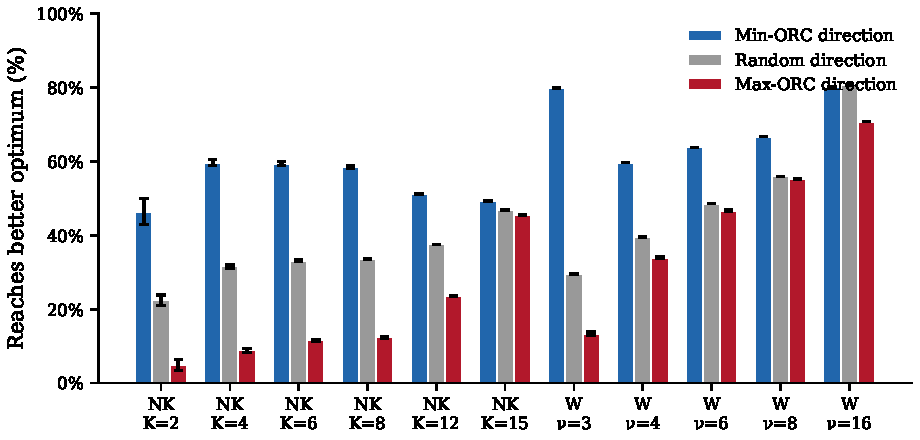
\includegraphics[width=\textwidth]{figures/fig_orc_advantage.pdf}
\caption{Fraction of local optima where following the min-ORC, random, or max-ORC (worst) direction leads to a strictly better local optimum. Error bars: standard error over 30 instances (N=16). The ORC advantage is largest at moderate ruggedness, where inter-basin transitions are neither trivial nor impossible.}
\label{fig:advantage}
\end{figure}

Figure~\ref{fig:advantage} shows the ORC advantage across all benchmark configurations.
A clear pattern emerges: the advantage is largest at \emph{moderate} ruggedness (NK $K = 4{-}8$, W-model $\nu = 3$) and diminishes toward both extremes.

This pattern is geometrically intuitive.
At low ruggedness ($K = 0{-}2$), the landscape has few optima and basin boundaries are obvious---even random perturbation finds improving directions.
At extreme ruggedness ($K = 15$, $\nu = 16$), the landscape is essentially random: all directions are equally (un)promising because the fitness function has no exploitable structure.
The ORC advantage peaks precisely in the ``interesting'' regime where the landscape has meaningful but non-trivial structure---the regime most relevant to practical optimization.

The W-model $\nu = 3$ result is particularly striking: ORC identifies improving directions in 79.9\% of cases while random direction succeeds only 29.4\% of the time (2.7$\times$ advantage), despite the HC success rate being a mere 0.3\%.
This demonstrates that ORC detects \emph{actionable} landscape structure that is invisible to global metrics.

\subsection{Results Scale to $N = 20$}

\begin{figure}[t]
\centering
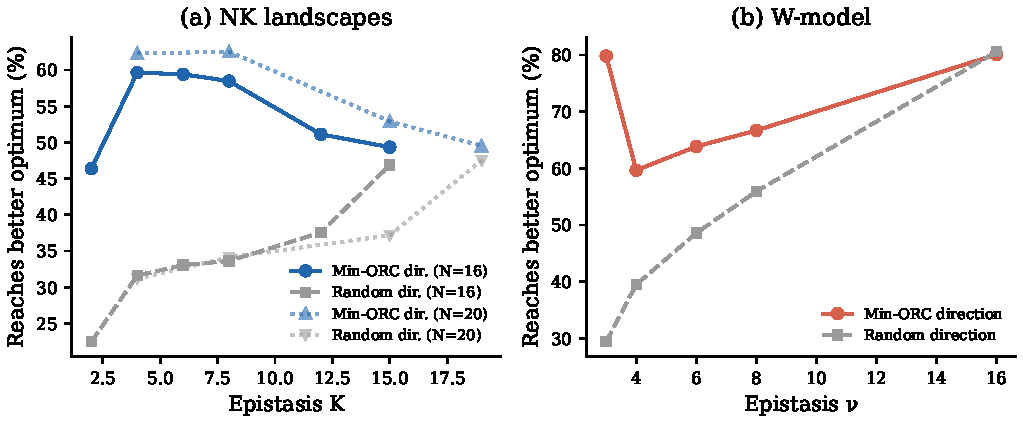
\includegraphics[width=\textwidth]{figures/fig_trends.pdf}
\caption{ORC advantage trends. (a)~NK landscapes: min-ORC vs.\ random direction success rate as a function of epistasis $K$, for both $N\!=\!16$ (solid) and $N\!=\!20$ (dotted). (b)~W-model: same comparison as a function of epistasis $\nu$. The ORC advantage is consistent across problem sizes.}
\label{fig:trends}
\end{figure}

A potential concern is that $N\!=\!16$ ($2^{16} = 65{,}536$ solutions) is a toy scale.
To address this, we ran the full analysis at $N\!=\!20$ ($2^{20} \approx 10^6$ solutions) for NK landscapes.
Table~\ref{tab:orc_summary} (middle rows) shows that the ORC advantage is \emph{at least as strong} at $N\!=\!20$: 62.3\% vs.\ 31.2\% at $K\!=\!4$ (2.0$\times$) and 62.5\% vs.\ 34.1\% at $K\!=\!8$ (1.8$\times$).

Figure~\ref{fig:trends}(a) confirms that the $N\!=\!20$ curves closely track the $N\!=\!16$ curves, suggesting that the ORC advantage is a robust structural property rather than a finite-size artifact.
Each $N\!=\!20$ instance requires about 60 seconds for full analysis (1M solutions, ORC at up to 50{,}000 local optima), demonstrating computational feasibility at non-trivial scales.

\subsection{ORC Correlates with Problem Difficulty}

\begin{figure}[t]
\centering
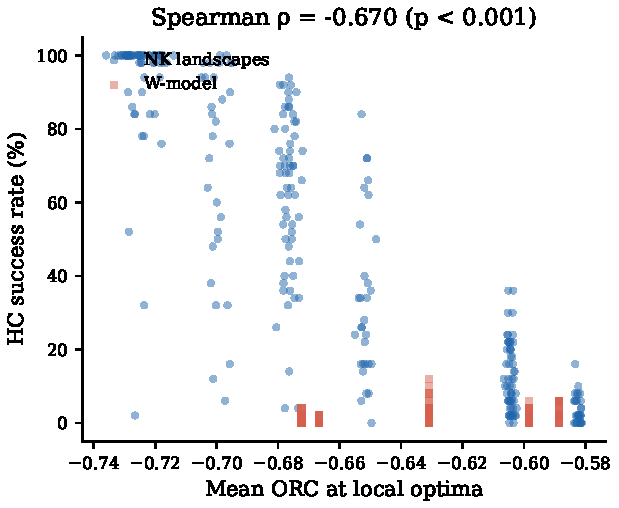
\includegraphics[width=0.55\textwidth]{figures/fig_scatter_orc_hc.pdf}
\caption{Mean ORC at local optima vs.\ HC success rate across 420 non-trivial instances ($N\!=\!16$). Each point is one instance, colored by benchmark type. More negative ORC (stronger neighborhood divergence) correlates with harder problems.}
\label{fig:scatter}
\end{figure}

\begin{table}[t]
\caption{Spearman rank correlations ($\rho$) between landscape metrics and algorithm performance across all 420 $N\!=\!16$ instances with $>1$ local optimum. $^{***}$: $p < 0.001$. The best value in each column is \textbf{bolded}.}
\label{tab:correlation}
\centering
\small
\begin{tabular}{@{}lrrr@{}}
\toprule
\textbf{Feature} & \textbf{HC success} & \textbf{EA success} & \textbf{RS mean fit.} \\
\midrule
Mean ORC (ours)               & $-0.670^{***}$ & $\mathbf{-0.652}^{***}$ & $-0.455^{***}$ \\
\%ORC$\to$better (ours)       & $-0.435^{***}$ & $-0.174^{***}$ & $-0.615^{***}$ \\
\%Rand$\to$better             & $-0.659^{***}$ & $-0.392^{***}$ & $-0.552^{***}$ \\
\midrule
FDC                           & $0.276^{***}$  & $0.501^{***}$  & $0.024$        \\
Autocorrelation length        & $0.543^{***}$  & $0.544^{***}$  & $0.372^{***}$  \\
Information content $H$       & $-0.308^{***}$ & $0.306^{***}$  & $-0.585^{***}$ \\
Basin entropy                 & $\mathbf{-0.731}^{***}$ & $-0.460^{***}$ & $\mathbf{-0.610}^{***}$ \\
\bottomrule
\end{tabular}
\end{table}

\begin{figure}[t]
\centering
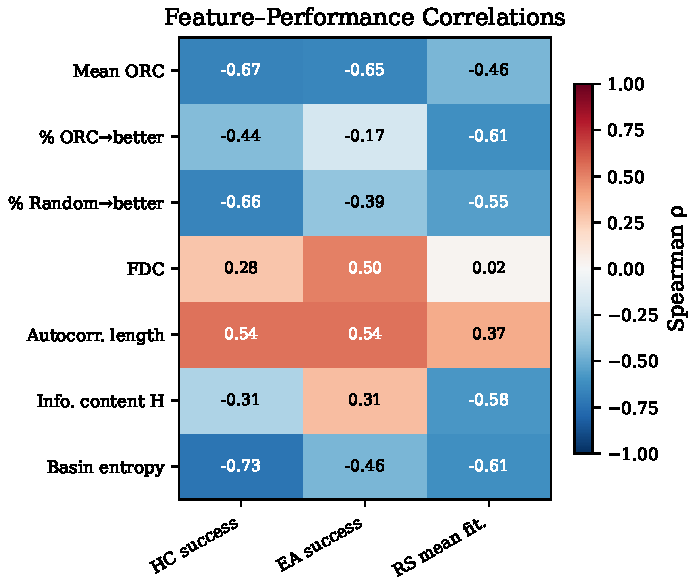
\includegraphics[width=0.65\textwidth]{figures/fig_correlation_heatmap.pdf}
\caption{Spearman rank correlations between all landscape metrics and algorithm performance targets. ORC-based features (top rows) show strong, consistent correlations across all targets, unlike FDC and information content which are inconsistent in sign.}
\label{fig:heatmap}
\end{figure}

Table~\ref{tab:correlation} and Figures~\ref{fig:scatter}--\ref{fig:heatmap} present the correlation analysis.
Key findings:

\begin{enumerate}
\item \textbf{Mean ORC} achieves the strongest correlation with HC difficulty ($\rho = {-}0.670$) among metrics that do not require full landscape enumeration, exceeding FDC~($0.276$) and information content~(${-}0.308$).
Only basin entropy ($\rho = {-}0.731$) is stronger, but it requires $O(2^N)$ evaluations and hill-climb operations---infeasible beyond $N\!\approx\!25$.
Mean ORC at $R$ sampled optima costs only~$O(R k^4)$, feasible at any scale.
Among tractable metrics, \textbf{Mean ORC is the strongest predictor across all three targets}.

\item \textbf{Mean ORC is consistently strong and sign-stable} across all three targets (HC, EA, RS), while classical metrics show inconsistent behavior.
Information content $H$ correlates \emph{negatively} with HC success but \emph{positively} with EA success, making it unreliable as a standalone predictor.
FDC has near-zero correlation with RS performance.

\item \textbf{\%Rand$\to$better} is itself a strong predictor ($\rho = {-}0.659$ for HC success, $\rho = {-}0.552$ for RS fitness), confirming that inter-basin transition probability is an important landscape property.
ORC's contribution is providing \emph{directional} information that significantly improves over random selection.
\end{enumerate}

\subsection{Comparison with Random-Interaction NK Landscapes}

\begin{table}[t]
\caption{Adjacent vs.\ random interaction NK landscapes ($N\!=\!16$). The ORC advantage is consistent across interaction models, though the random model produces fewer local optima at equal $K$.}
\label{tab:interaction}
\centering
\small
\begin{tabular}{@{}llrrrr@{}}
\toprule
$K$ & \textbf{Model} & \textbf{\#Opt.} & \textbf{\%ORC} & \textbf{\%Rand} & \textbf{Adv.} \\
\midrule
2   & adjacent & 31   & 46.4 & 22.5 & 2.1$\times$ \\
2   & random   & 24   & 42.8 & 20.3 & 2.1$\times$ \\
\midrule
6   & adjacent & 463  & 59.4 & 33.1 & 1.8$\times$ \\
6   & random   & 364  & 56.6 & 26.8 & 2.1$\times$ \\
\midrule
12  & adjacent & 2249 & 51.1 & 37.6 & 1.4$\times$ \\
12  & random   & 2176 & 51.0 & 37.3 & 1.4$\times$ \\
\bottomrule
\end{tabular}
\end{table}

To verify that our results are not specific to the adjacent interaction model, Table~\ref{tab:interaction} compares NK landscapes with adjacent and random interaction.
The ORC advantage is remarkably consistent across models: at $K = 6$, the advantage is 1.8$\times$ (adjacent) vs.\ 2.1$\times$ (random).
The random model produces slightly fewer local optima at equal $K$ but the same qualitative ORC behavior, confirming the generality of our findings.

\subsection{ORC Reveals Structure Invisible to Classical Metrics}

Unlike FDC and autocorrelation, which produce a single number per instance, ORC provides \emph{per-local-optimum} directional information: which neighbor leads out of the current basin, how strongly each direction diverges, and the heterogeneity of escape difficulty across optima.
By recording which optimum each negative-ORC direction leads to, one can construct an \emph{ORC transition graph}---a deterministic, curvature-weighted analogue of stochastic LON transition edges.


% ===================================================================
\section{Discussion}
\label{sec:discussion}
% ===================================================================

\subsection{Why the ORC Advantage Diminishes at High Ruggedness}

At $K = 15$ (NK) and $\nu = 16$ (W-model), the ORC advantage over random direction nearly vanishes (Table~\ref{tab:orc_summary}).
This is expected: maximally rugged landscapes ($K = N - 1$) have fitness values that are essentially independent random variables at each solution.
When there is no exploitable fitness structure, \emph{no} metric can identify productive directions---ORC, FDC, and random direction all converge to the same baseline.
The persistence of the ORC advantage at intermediate ruggedness ($K = 4{-}8$, $\nu = 3{-}6$) is the practically relevant finding, as real-world problems typically exhibit moderate, not maximal, ruggedness.

\subsection{Sensitivity to $\gamma$}

The fitness sensitivity parameter $\gamma$ controls the relative weight of fitness differences in the transport cost~\eqref{eq:lifted}.
To verify that our findings are not an artifact of the specific choice $\gamma = 1$, we repeated the full analysis at $\gamma \in \{0.1, 0.5, 1.0, 2.0\}$ for NK landscapes ($N\!=\!16$, $K \in \{4, 8, 12\}$, 30 instances each).
The ORC advantage is effectively invariant: \%ORC and the advantage ratio remain constant across all tested $\gamma$ values (e.g., $59.6\%$ vs.\ $31.6\%$ at $K\!=\!4$ for every $\gamma$, giving a stable $1.9\times$ advantage).
This robustness is explained by Theorem~\ref{thm:negative}: the negative ORC arises primarily from the overlap structure of the neighborhoods (the $\delta$ terms), not from the fitness-difference terms ($\gamma\,|f(a)\!-\!f(b)|$).
Since the overlap structure is a graph-topological property independent of $\gamma$, the curvature sign and the resulting escape-direction ranking are insensitive to the choice of $\gamma$.

\subsection{Relation to Local Optima Networks}

Our ORC transition graph shares structural similarities with LONs~\cite{ochoa2008first,ochoa2017understanding}, but LON edges are discovered via stochastic perturbation-climb cycles capturing \emph{reachability}, whereas ORC edges are computed deterministically and capture \emph{geometric preference}.
Combining both views---using ORC to weight LON edges---is a promising direction for future work.

\subsection{Practical Implications for Algorithm Design}

Our results suggest two immediate applications:
\begin{enumerate}
\item \textbf{ORC-guided escape.} At a local optimum, following the min-ORC direction leads to improvement $1.4{-}2.7\times$ more often than following a random neighbor (Table~\ref{tab:orc_summary}).
Since the min-ORC direction is deterministic, a multi-step ORC-guided search should randomize among \emph{all} negative-ORC directions (not just the minimum) to avoid cycling.
\item \textbf{ORC as an algorithm selection feature.} Mean ORC at sampled local optima ($\rho = {-}0.670$ with HC success) provides a strong, computationally tractable predictor of hill-climbing difficulty, complementing existing ELA features.
\end{enumerate}

\subsection{Limitations}

\textbf{Scale and neighborhood size.}
Full landscape enumeration is feasible at $N\!=\!20$ (${\sim}60$\,s) but not beyond; a sampling-based approach computing ORC at optima found by repeated hill climbing suffices for larger~$N$, since the per-optimum cost is~$O(k^4)$.
For $k \gg 100$, subsampling the support distributions would be needed.

\textbf{Graph structure.} Theorem~\ref{thm:negative} assumes the binary hypercube ($N \ge 4$) where adjacent nodes share no common neighbors; it extends to any $k$-regular graph with disjoint exclusive neighborhoods, verified on NAS-Bench-201 ($k\!=\!24$).
Extending the result to plateaus remains open, though negative ORC is observed at all local optima empirically.


% ===================================================================
\section{Conclusion}
\label{sec:conclusion}
% ===================================================================

We have introduced Ollivier--Ricci curvature as a landscape metric for discrete combinatorial optimization.
Our main finding is that the most-negative-ORC direction at a local optimum leads to a better basin $1.4{-}2.7\times$ more often than a random direction, across 530+ benchmark instances spanning NK landscapes, the W-model, and NAS-Bench-201.
This advantage is supported by a rigorous theoretical guarantee---an explicit sufficient condition for negative ORC (Theorem~\ref{thm:negative}) satisfied at 100\% of tested optima---and holds at both $N\!=\!16$ and $N\!=\!20$ scales.

ORC offers three capabilities absent from existing metrics:
(1)~per-optimum \emph{directional} escape information;
(2)~a \emph{geometric} account of basin connectivity via optimal transport;
and (3)~strong correlation with algorithm difficulty, surpassing FDC and autocorrelation.

Future work includes:
(a)~integrating ORC into adaptive search operators for practical optimization;
(b)~developing sampling-based ORC for large-scale landscapes;
(c)~combining ORC with LON analysis for richer landscape characterization; and
(d)~extending ORC to permutation and other non-binary search spaces.

\paragraph{Reproducibility.} All code and data are available at \url{[anonymized]}.


% ===================================================================
% References
% ===================================================================

\begin{thebibliography}{99}

\bibitem{dong2020bench}
Dong, X., Yang, Y.: NAS-Bench-201: Extending the scope of reproducible neural architecture search. In: ICLR (2020)

\bibitem{dong2021nats}
Dong, X., Liu, L., Musber, K., Graves, B., Shivakumar, P., Yang, Y.: NATS-Bench: Benchmarking NAS algorithms for architecture topology and size. IEEE TPAMI \textbf{44}(7), 3634--3646 (2021)

\bibitem{jones1995fitness}
Jones, T., Forrest, S.: Fitness distance correlation as a measure of problem difficulty for genetic algorithms. In: ICGA, pp.~184--192 (1995)

\bibitem{kauffman1993origins}
Kauffman, S.A.: The Origins of Order: Self-Organization and Selection in Evolution. Oxford University Press (1993)

\bibitem{kerschke2019automated}
Kerschke, P., Hoos, H.H., Neumann, F., Trautmann, H.: Automated algorithm selection: Survey and perspectives. Evolutionary Computation \textbf{27}(1), 3--45 (2019)

\bibitem{kuhn1955hungarian}
Kuhn, H.W.: The Hungarian method for the assignment problem. Naval Research Logistics Quarterly \textbf{2}(1--2), 83--97 (1955)

\bibitem{mersmann2011exploratory}
Mersmann, O., Bischl, B., Trautmann, H., Preuss, M., Weihs, C., Rudolph, G.: Exploratory landscape analysis. In: GECCO, pp.~829--836. ACM (2011)

\bibitem{ni2019community}
Ni, C.C., Lin, Y.Y., Luo, F., Gao, J.: Community detection on networks with Ricci flow. Scientific Reports \textbf{9}, 9984 (2019)

\bibitem{ochoa2008first}
Ochoa, G., Tomassini, M., V\'erel, S., Darabos, C.: A study of NK landscapes' basins and local optima networks. In: GECCO, pp.~555--562. ACM (2008)

\bibitem{ochoa2014local}
Ochoa, G., Veerapen, N.: Deconstructing the Big Valley search space hypothesis. In: EvoCOP. LNCS, vol.~8600, pp.~58--69. Springer (2014)

\bibitem{ochoa2017understanding}
Ochoa, G., Veerapen, N., Daolio, F., Tomassini, M.: Understanding phase transitions with local optima networks: Number partitioning as a case study. In: EvoCOP. LNCS, vol.~10197, pp.~233--248. Springer (2017)

\bibitem{ollivier2009ricci}
Ollivier, Y.: Ricci curvature of Markov chains on metric spaces. Journal of Functional Analysis \textbf{256}(3), 810--864 (2009)

\bibitem{pitzer2012comprehensive}
Pitzer, E., Affenzeller, M.: A comprehensive survey on fitness landscape analysis. In: Recent Advances in Intelligent Engineering Systems, pp.~161--191. Springer (2012)

\bibitem{sandhu2015graph}
Sandhu, R., Georgiou, T., Reznik, E., Zhu, L., Kolesov, I., Senbabaoglu, Y., Tannenbaum, A.: Graph curvature for differentiating cancer networks. Scientific Reports \textbf{5}, 12323 (2015)

\bibitem{stadler1996landscapes}
Stadler, P.F.: Landscapes and their correlation functions. Journal of Mathematical Chemistry \textbf{20}, 1--45 (1996)

\bibitem{topping2022understanding}
Topping, J., Di~Giovanni, F., Chamberlain, B.P., Dong, X., Bronstein, M.M.: Understanding over-squashing and bottlenecks on graphs via curvature. In: ICLR (2022)

\bibitem{vassilev2000information}
Vassilev, V.K., Fogarty, T.C., Miller, J.F.: Information characteristics and the structure of landscapes. Evolutionary Computation \textbf{8}(1), 31--60 (2000)

\bibitem{villani2009optimal}
Villani, C.: Optimal Transport: Old and New. Springer (2009)

\bibitem{weise2014difficult}
Weise, T., Wu, Z.: Difficult features of combinatorial optimization problems and algorithm selection with the W-model. In: GECCO Companion, pp.~1453--1460. ACM (2014)

\end{thebibliography}

\end{document}
